\documentclass[12pt]{article}
% Essential packages
\usepackage{tikz}
\usepackage{pgfplots}
\usepackage[utf8]{inputenc}
\usepackage{graphicx}
\usepackage{amsmath}
\usepackage{cite}
\bibliographystyle{plain}
\usepackage{hyperref}
\usepackage{amsmath}
\usepackage{graphicx}
\usepackage{hyperref}
\usepackage{geometry}
\geometry{a4paper, margin=1in}

% TikZ and PGF plots configuration
\pgfplotsset{compat=1.18}
\usetikzlibrary{arrows,shapes,positioning,calc}

\begin{document}
\title{Evolution of Cloud Computing Systems: \\
From General Frameworks to Specialized Solutions}

\author{\\\textbf{\ Hu Silan}\\A0304367E \and \\\textbf{\ Wang Zhaoyu}\\A0290549U }
\maketitle

\section{Introduction}

Cloud computing has changed how we process big data. But there is still a main problem: how to make distributed systems that are both efficient and easy to program. This problem exists because it's hard to make systems simple to use while also making them work very fast. MapReduce \cite{dean2008mapreduce} showed a good way to solve this by breaking distributed computation into two simple steps: map and reduce. This made it easier for normal developers to write distributed programs. But this simple approach had a big problem - by treating computation like a black box, it moved too much data around and wasted resources. Research shows that in real systems, almost half (47\%) of I/O operations were just moving data \cite{olston2008pig}.

The field's response to this problem has been interesting. Instead of trying to find one solution for everything, system designers started making optimizations for specific types of work - but in a special way. New systems work well because they deeply understand specific types of workloads, while still being easy to program. For example, Arabesque \cite{teixeira2015arabesque}, which was made for analyzing graphs, uses a computation model that matches well with how graph algorithms work. This makes it much faster while still being easy to use.

This change has gotten faster in recent years. Meta's XFaaS \cite{shahrad2020serverless} shows why this approach is so important when working at very large scale - when processing trillions of function calls every day, even small inefficiencies can cost a lot. Their specialized scheduling system achieves 66\% CPU usage while staying easy to program, which is much better than traditional schedulers. Also, new research in microsecond-scale computing \cite{barroso2017attack} shows how specialized scheduling can keep response times very fast while handling lots of data.

These findings show something important: systems can be both efficient and easy to program if we find the right way to design them for specific problems. As Figure 1 shows, systems made for specific domains can get close to the best possible performance while still being easy to use. This is a big change in how we design cloud systems. This paper looks at how cloud computing has changed by studying five important systems from the last 20 years. We look at how systems have moved from general-purpose to specialized solutions. We identify what worked well and what problems still exist, especially focusing on how systems handle trade-offs in big data environments and what this means for future cloud system design.

\begin{figure}[t]
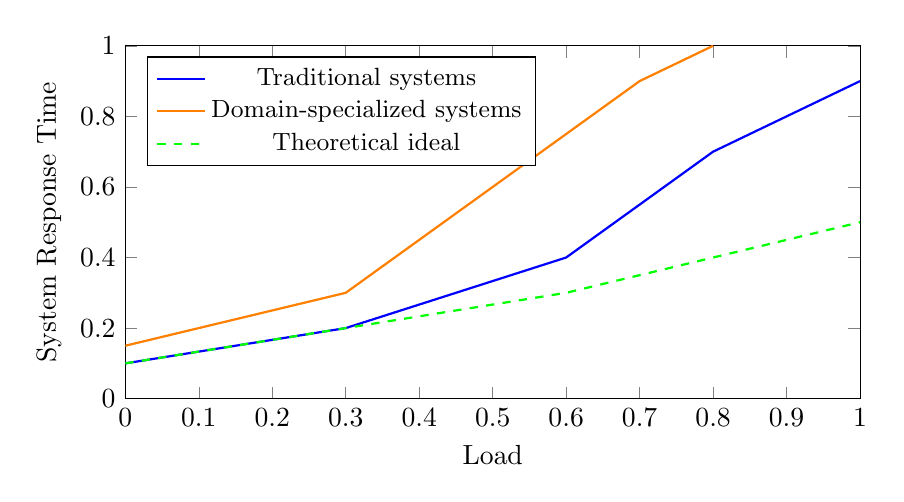
\begin{tikzpicture}
\begin{axis}[
    xlabel=Load,
    ylabel=System Response Time,
    xmin=0, xmax=1,
    ymin=0, ymax=1,
    width=0.9\textwidth,
    height=0.5\textwidth,
    legend pos=north west,
    legend style={font=\small}
]
\addplot[blue, thick] coordinates {
    (0,0.1) (0.3,0.2) (0.6,0.4) (0.8,0.7) (1,0.9)
};
\addplot[orange, thick] coordinates {
    (0,0.15) (0.3,0.3) (0.5,0.6) (0.7,0.9) (0.8,1)
};
\addplot[green, thick, dashed] coordinates {
    (0,0.1) (0.3,0.2) (0.6,0.3) (0.8,0.4) (1,0.5)
};
\legend{Traditional systems,Domain-specialized systems,Theoretical ideal}
\end{axis}
\end{tikzpicture}
\caption{The evolution of cloud system design: While traditional systems faced sharp performance degradation under load, modern domain-specialized systems approach theoretical ideals through careful optimization and approximation.}
\label{fig:tradeoff}
\end{figure}

\section{Fundamental Concepts and Models}

\subsection{How Distributed Abstraction Started: MapReduce}
MapReduce \cite{dean2008mapreduce} changed distributed computing by introducing a simple two-function programming model. Before this, developers had to handle complex problems like parallelization, fault tolerance, and data distribution themselves. The model was good because it was simple: developers only needed to write two main functions, and the system handled everything else. MapReduce influenced many other systems \cite{isard2007dryad}, and changed how we think about data processing and distributed computing.

But this simplicity had problems. MapReduce made things simple by treating computation as a black box. User-Defined Functions (UDFs) contained user code but hid opportunities to make things faster. The performance cost was big - moving data around used up to 47\% of I/O in real systems \cite{olston2008pig}. This showed a basic problem: making things simple often means making them less efficient.

\subsection{Making User-Defined Functions Better}
Researchers saw the problems with black-box UDFs and tried to find better solutions. New systems like CIEL \cite{murray2011ciel} introduced new ways to analyze how UDFs work to move data more efficiently and waste fewer resources. This change in how we think about UDFs was very important - it showed we could make things faster without making them harder to program.

\subsection{The Rise of Domain-Specific Systems}
As data got more complex, it became clear that one general solution couldn't handle all types of problems well. This led to the development of specialized systems for specific types of work.

For graph processing, systems like Pregel \cite{malewicz2010pregel} introduced the "Think Like a Vertex" idea, where computations are organized from the view of individual vertices. This changed how we do distributed graph processing and made it easier to write algorithms. But this approach wasn't good enough for more complex tasks like pattern mining.

Arabesque \cite{teixeira2015arabesque} is a good example of a domain-specific system for graph mining. It introduced the "Think Like an Embedding" (TLE) approach, which works well with graph algorithm patterns. By treating subgraphs as main parts of the system, Arabesque made it possible to efficiently explore huge graphs while being easier to use.

\subsection{Managing Trade-offs and Measurements}
The change from MapReduce to systems like CIEL and Arabesque shows important trade-offs in cloud system design. One big challenge is managing tail latency, as Dean and Barroso \cite{dean2013tail} showed how variations in response time can seriously affect service quality. This understanding has led to new ways of designing systems and managing resources.

These trade-offs have real effects. For example, I/O inefficiencies in real systems can cause big performance problems and increase costs \cite{atikoglu2012workload}. Modern systems must balance these competing needs while still being able to handle growth.

\subsection{Almost Perfect Performance and Microsecond Response Times}
Recent advances focus on getting very close to the best possible performance. Microsecond-scale response times have become very important for modern data centers, as shown in "Attack of the Killer Microseconds" \cite{barroso2017attack}. This research showed how delays of just microseconds can significantly affect system performance.
Research by Kaffes et al. \cite{kaffes2019shinjuku} shows ways to get very fast response times through smart scheduling. These methods show how systems can get close to the best possible performance without needing to be perfect.

\subsection{Serverless Computing at Very Large Scale}
Serverless computing brings new challenges to system design. As Li et al. \cite{li2022serverless} explain, serverless platforms handle infrastructure management so developers can focus on writing application code. But running these systems at large scale creates unique problems, as shown by Meta's XFaaS experience \cite{shahrad2020serverless}.

Shahrad et al. \cite{shahrad2020serverless} studied serverless workloads at large scale and found challenges in handling sudden increases in load and cold starts. These challenges have led to new developments in lightweight virtualization, like Firecracker \cite{agache2020firecracker}.

Meta's experience with large systems, including TAO \cite{bronson2013tao} and their real-time platform \cite{chen2016realtime}, shows how important it is to handle data and computation efficiently at large scale. These systems show how modern architectures can handle huge workloads while maintaining good performance and reliability.

\subsection{New Design Patterns and Models}
Looking at all these systems shows new patterns and challenges, especially in microservices architectures \cite{gan2019open}, \cite{netflix_microservices}. The field keeps changing, with research focusing on:

\begin{itemize}
\item \textbf{Domain-Aware Design:} Systems increasingly use domain-specific knowledge while staying easy to use \cite{gonzalez2012powergraph, elseidy2014grami, jahani2011optimization}.

\item \textbf{Microsecond Performance:} Managing microsecond-scale delays \cite{barroso2017attack, dean2013tail} has become crucial for modern data centers. As demonstrated by Shinjuku \cite{kaffes2019shinjuku}, careful scheduling is essential for achieving microsecond-scale tail latency.

\item \textbf{Resource Efficiency:} As shown by modern serverless systems \cite{shahrad2020serverless, agache2020firecracker}, using resources well remains critical. Studies of production workloads \cite{atikoglu2012workload, cao2020rocksdb} demonstrate the importance of efficient resource utilization.

\item \textbf{Ability to Grow:} Modern systems must handle bigger workloads while maintaining performance, as shown by large-scale deployments \cite{chen2016realtime, bronson2013tao}.
\end{itemize}

New advances in serverless computing \cite{jonas2019cloud, li2022serverless} suggest cloud programming will become easier to use while still being fast enough. These developments show we're moving toward systems that successfully balance usability and efficiency \cite{mcsherry2015scalability}, learning from past experiences while solving new challenges.

\section{MapReduce Paradigm and Data Flow Optimization}

MapReduce's creation was a very important moment in cloud system design. It first showed how to balance two things that seemed impossible to combine: making systems easy to use and making them work well. This section looks at how MapReduce was designed and how later improvements in data transfer made the foundation for domain-specific systems.

\subsection{How MapReduce Was Designed and Built}
When Dean and Ghemawat created MapReduce, they had a big challenge: how to help normal programmers write programs that could run on thousands of computers. Their solution followed a simple idea - make things as simple as possible. They broke down distributed computing into just two operations: map and reduce. This simple approach had deep wisdom behind it: by limiting how programmers could write programs, the system could automatically handle the most difficult parts of distributed computing.

The execution flow shown in Figure~\ref{fig:mr_flow} shows how well it was designed:

\begin{figure}
    \centering
    \includegraphics[width=0.5\linewidth]{MapReduce_Execution_overview.png}
    \caption{Execution overview of MapReduce}
    \label{fig:mr_flow}
\end{figure}

As shown in \cite{dean2008mapreduce}, MapReduce became very successful at Google - from 2004 to 2008, the number of MapReduce programs at Google went from zero to thousands. This success happened mainly because it could handle growth very well. By splitting input data into fixed-size pieces (usually 16-64MB), MapReduce could grow almost linearly. Tests showed it could sort 1TB of data in just minutes \cite{dean2008mapreduce}.

\subsection{Making Data Transfer Better}
However, MapReduce's simple design also had problems. The biggest problem was that it moved data inefficiently - because User Defined Functions (UDFs) were treated like black boxes, the system couldn't optimize how data moved between map and reduce phases. This was a big problem in real applications, where moving data could use up 47\% of all I/O operations \cite{olston2008pig}.

This problem led to important improvements. The most important was the SUDO framework, which introduced UDF-aware optimization \cite{jahani2011optimization}. By studying how UDFs worked, SUDO could predict how data would flow and organize data better. This made data transfer much more efficient while keeping MapReduce simple to use.

Importantly, these improvements provided good ideas for later domain-specific systems. For example, the "Think Like an Embedding" approach used by Arabesque \cite{teixeira2015arabesque} in graph computing can be seen as taking the MapReduce model and making it better for a specific type of work. This shows that by deeply understanding specific types of computation, we can make systems work better while keeping them easy to use.

\subsection{Effects and What We Learned}
MapReduce and the research to improve it had big effects on how cloud systems are designed:

\begin{enumerate}
\item \textbf{Good Design Matters}: MapReduce showed that well-designed systems could make distributed programming much simpler while still working well enough. This idea influenced many later systems.

\item \textbf{Balance Between Performance and Ease of Use}: Research on data transfer showed that systems could do complex optimizations in lower layers while keeping things simple for programmers to use. This helped later designers make domain-specific systems.

\item \textbf{Ability to Grow}: How MapReduce split data and handled failures set standards for building large distributed systems, and these lessons are still useful in modern systems.
\end{enumerate}

New developments in serverless computing \cite{jonas2019cloud} and microsecond-scale computing \cite{barroso2017attack} continue to build on these ideas. As shown by Meta's XFaaS \cite{shahrad2020serverless}, modern systems can use resources better (66\% CPU usage) while staying simple to program by using specialized improvements.

Looking at how MapReduce has changed, we see an important trend: system design is moving from general approaches toward domain-specific approaches. This change keeps the benefits of being easy to use while getting better performance through deeper understanding of specific domains. As shown by modern systems like Arabesque \cite{teixeira2015arabesque} and Shinjuku \cite{kaffes2019shinjuku}, this suggests where cloud computing systems are going: making performance better through deeper understanding of specific domains while keeping things simple.

\newpage
\bibliography{silan-reference}
\end{document}
